% chap7.tex - Week 7
\cleardoublepage
%\phantomsection
\chapter{Week 7}

\section{Day 1 - ``Networking with a difference''}
\subsection{Pushing across a LAN}

\index{SSH}Now we have a complete copy of our repository in another location.
At the moment we have created this clone on the same machine that our original is.
This isn't really a very good idea for backup purposes.
Git supplies several means with which to talk to a remote machine, but by far the most common of these is to utilise the SSH protocol.
SSH is a secure, encrypted way to communicate with a remote repository.
Which is a must for pushing to an important repository that people are going to pull information from.

If we assume that for a moment that our user \emph{john} has now moved to another machine and now wishes to clone a repository that he had on his original machine to this new one.
The commands are identical to that which we used before.
We are going to assume that \emph{john} already has SSH access to the machine.
In this way, we can issue the commands as follows.

\begin{code}
john@akira:~$ git clone ssh://john@satsuki/home/john/coderepo coderepo-ne
Initialized empty Git repository in /home/john/coderepo-ne/.git/
john@akira's password:
remote: Counting objects: 53, done.
remote: Compressing objects: 100% (36/36), done.
Receiving objects: 100% (53/53), 4.84 KiB, done.
Resolving deltas: 100% (10/10), done.
remote: Total 53 (delta 10), reused 0 (delta 0)
john@akira:~$
\end{code}

Now we have done exactly as before and cloned our repository to a local folder called \texttt{coderepo-ne} from the remote URL \texttt{ssh://john@satsuki/home/john/coderepo}.
Notice the use of \texttt{ssh://} to denote the specification of the SSH protocol.
We have also put the users name in the URL of the remote path.
If the SSH server was running on a different port to usual, that is, on a port other than 22, we could have also added a port number preceded by a colon after the hostname.

\index{Git!Protocol}SSH isn't the only protocol that Git can use.
We have already looked at two; local and SSH.
In fact, Git supports a further two protocols and these are HTTP/S and Git's own GIT protocol.
We are going to take a quick look at the Git protocol next, before moving on to HTTP/S.

\subsection{The Git Protocol}
The GIT protocol is the fastest transfer protocol out there for Git repositories.
This should come as no surprise, since it was developed exclusively for use within a Git environment.
It does however have a relatively large drawback.
The drawback is that it provides absolutely no authentication.
For this reason, enabling the GIT protocol on a repository and running the server back-end, (described later), will allow anyone who can talk to the servers port complete read access to the repository.

If you are serving a large repository on the Internet for example, this could actually be rather beneficial and will allow you to serve pulls quickly and efficiently.
However, though it is possible to enable \emph{pushing} using the GIT protocol, the lack of security would mean that anyone who could see the server and connect to the port, usually 9418, could make changes to the repository.
This is usually entirely undesirable and as such people will often couple a read-only GIT protocol with a writable SSH protocol for the developers that need push access.

\subsection{The HTTP/S Protocol}
\index{HTTP/S Protocol}Just as with the GIT protocol, Git can support the HTTP/HTTPS protocol as well.
Setting up this is usually as simple as creating a bare clone of your repository, keeping it up to date, usually via a post-update-hook, which is described later in the book, and simply allowing clients access to this server area.

Note that the above is only to provide read-only access over HTTP.
It is possible to allow write access, i.e.\ pushing, over HTTPS, but this is more complicated to set up and is outside the scope of this book.

\subsection{Protocol decision}
\index{protocol decision}Tamagoyaki are about to embark on their decision making process regarding which protocols to use and how to perform their collaboration between themselves and their external partners.
They are going to have to take multiple things into consideration, such as security, speed, administration and storage.
When you begin to implement the Git system yourself, you too will have to think about these decisions and answer questions like:

\begin{itemize}
\item Who is going to require access to the repository?
\item How many people are going to require access to the repository?
\item Is the information sensitive, either from an IP perspective or from a customer point of view?
\item How large is the data that we are hosting?
\item How large is the change set?
\item Do we need a QA area?
\item Do we need a Production area?
\end{itemize}

This is just a short list of the questions that you will need to consider when implementing a full on Git environment.
The beauty of the Git system though, is that it is flexible and very difficult to box yourself into a corner, where a decision made early on prohibits a different approach later on.

\section{Day 2 - ``Now let's work together''}
\subsection{Pure collaboration}

We are now armed with a much clearer idea of how Git works and indeed we are now in a position to actually implement the developmental model that the team of Tamagoyaki need in order to collaborate on their projects.
It should be noted that although we have reached the point of being able to work together on a project, this is not where out discussions about Git will end.
We still have a number of topics to cover and these will be visited as required during the subsequent implementation of Git at Tamagoyaki.

\begin{trenches}
``So I still maintain that we follow the original plan,'' said Rob.
``Each person has their own repository and is the master of their own commits''

John shook his head.
``On a small scale,'' he began,
``that might work.''
He paused for a breath.
``But we need to think about scalability too. Whilst I don't think all development work should be in one repository, I also don't think the best way to go is to have a repo for every person.''

``I know it's a rarity, but I gotta agree with John.'' Klaus spoke whilst idly stabbing his pen lightly into a blob of what looked like modelling clay.
``Think what the chimp would say to it too.''

Martha furrowed her brow,
``The chimp?'' she asked.

John turned to look at Martha and almost regretted having to inform her of yet another of Klaus' pet names.
``That's what Klaus calls Jimmy in IT.''

Martha looked a little horrified,
``Klaus, that's an awful thing to say.''

``What? He spends all day monkeying around in the 'datacenter'. I've never really seen him do any real work at all.''
Klaus was looking at Martha who now had one eyebrow raised.
He had used air quotes when voicing the word 'datacenter'.
``Plus he calls it a datacenter, but I've seen inside, it's more like a cupboard with a PC in it.''

``You need to show a little more respect Klaus,'' Martha threw back, a little more aggressively than she had intended.

``Guys!! Guys!!'' John shouted.
``Can we get back to the topic at hand and deal with Klaus later?''

The room fell silent for a while, until the comments had transitioned from immediate to short term memory.
``How about doing it by team?''
It was Eugene speaking now.
``You know, kinda like a Mob repository. Each team will have their own repository and the branches inside will belong to the different team members and be named accordingly so. Then we would have a company repository which would hold the projects and would have dev, qa and released branches.''

``You know that's not a bad idea Eugene.'' Klaus said, trying to redeem himself.
``You da man. How about a hi-five.''

\end{trenches}

\index{mob repository}The idea of having a Mob repository is not anything new.
Many people decide to split up their teams in this way especially within a company.
For larger repositories it makes a lot of sense as not only does it help to keep development altogether in one place, but it also saves on space and administration overhead.
Managing many smaller repositories is often a lot more time consuming than managing several larger ones.

However you should always look at the situation and the scenario carefully to see which is going to suit you best.
For Tamagoyaki, there is the prospect of the teams growing soon and so they require a way to get the data organised fairly quickly and effortlessly.
Having many small repositories would likely confuse new members to the team, so the decision to move forward with team based and site based repositories makes sense.

\index{blessed repository}Tamagoyaki are proposing to have a single repository which will be the \emph{blessed} repository we discussed way back at the beginning of the book.
This repository will likely hold three branches.
These will relate to development, quality assurance and releases.
To this end it will allow one team to gain access to features that the other teams are working on, via the development branch.
It will allow a QA manager to work on the quality assurance branch and finally, it will allow someone to push these changes through to the released branch.

The idea is that all development work stays in the development branch.
For Tamagoyaki Inc.
this branch will likely contain mostly finished, but largely untested works.
The teams will work together inside their mob repositories to create new functionality.
Once they are happy, their team leader will push their changes up into the development branch on the \emph{blessed} repository.
This branch is not guaranteed to be stable.
Sometimes things will break but the development branch is a place that all of the work of the various teams comes together.

Once the teams hit feature freeze, the point at which they will no longer take any more new features into the code base, they will ask the QA manager to create a \textbf{QA} branch.
Bug fixes for current issues will be committed here and when all bugs have been fixed and the code is ready to be released, the release branch will be synced with a specific commit of the \textbf{QA} branch.

If this all sounds a little confusing, we will take a few minutes to digest what we have come up with and draw a few diagrams.
The beauty of Git is that it is so configurable and so by design supports almost limitless workflows.
Unfortunately this can also be a drawback because no two Git setups are generally alike.
The set up of Git is totally customised to the situation or scenario at hand.
In our case, we have merged together two of the workflow models that we presented in the early chapters.

\begin{figure}[hbt]
\centering
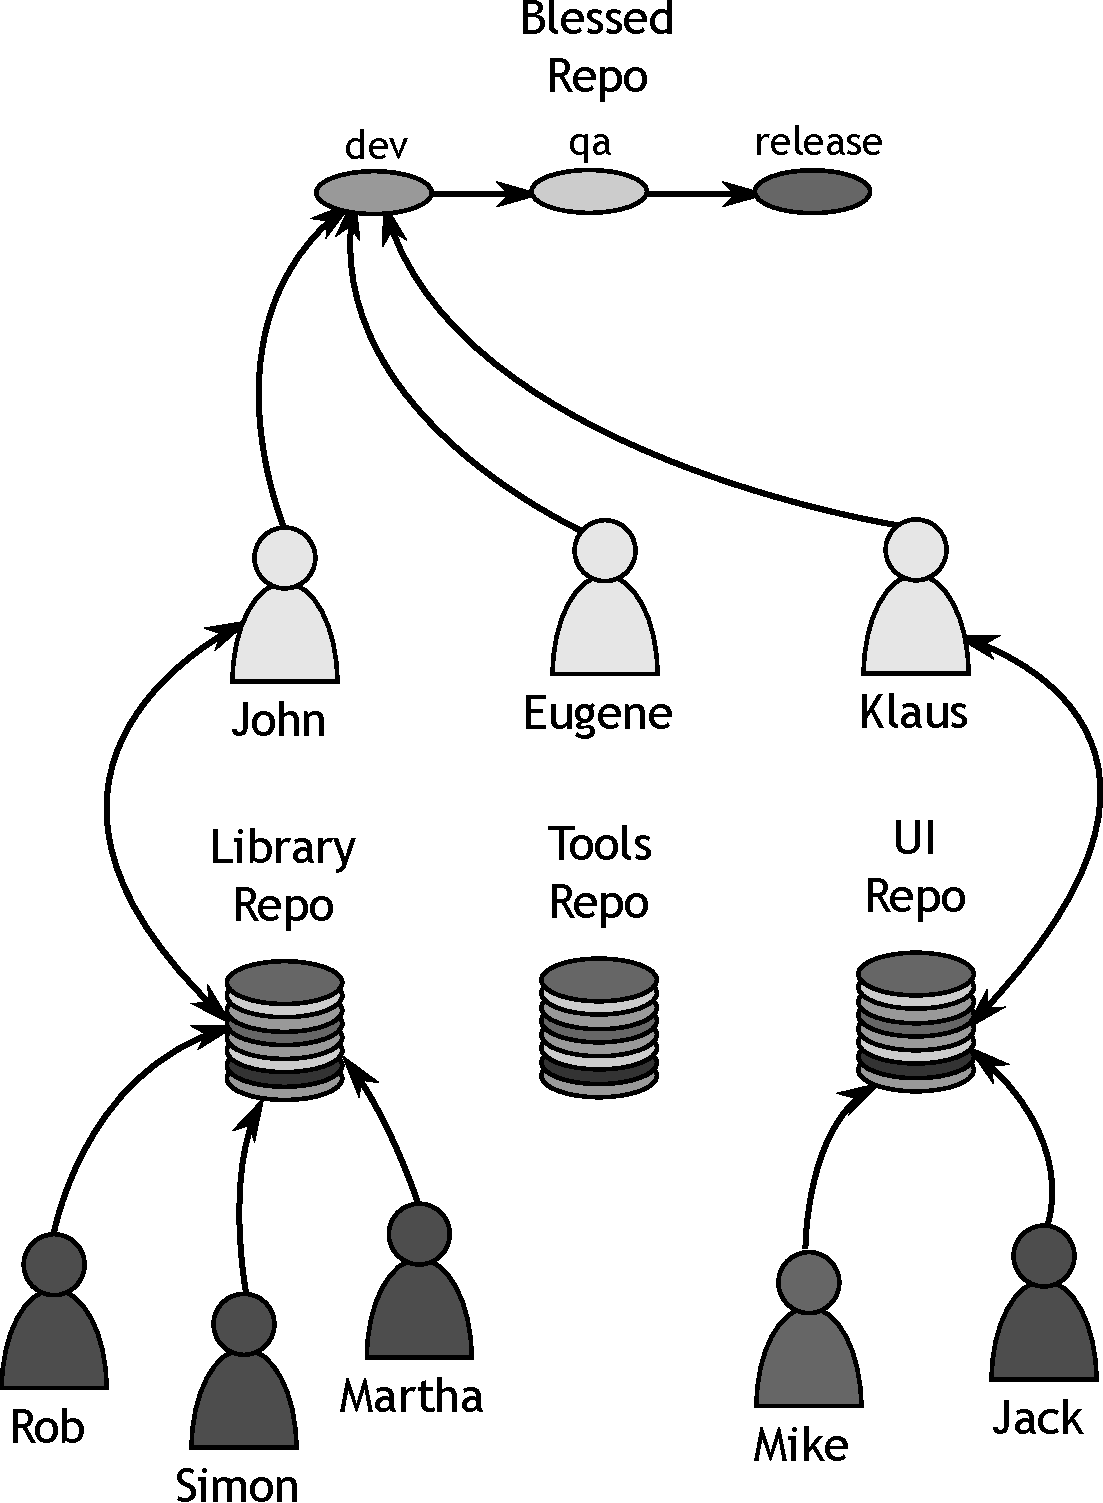
\includegraphics[width=9cm]{images/f-w7-d1.pdf}
\caption{Our workflow}
\end{figure}

We are using a \emph{blessed} repository with which to store our crown jewels.
This is the repository that contains our main \textbf{release} branch.
This branch will always contain reliable stable releases.
Sure, it may contain history of how we reached the stable release, but on a checkout, it will be a solid, buildable, pristine, tagged release.
This repository also contains our \textbf{QA} branch.
This is the branch that upon checkout would contain a fairly polished version of the product, but it may still have a few bugs and issues.
Then we have our development branch.
This is where the integration managers from the various teams would pull the code from their teams into a single code base, ready for the QA manager to begin his testing.
This setup may not work for you.
You may require more levels, you may require less.
The fact of the matter is that Git allows you to make that distinction.

For the developers, we have the team mob repositories.
These repositories will contain multiple branches that the various team members will push to, so that the integration managers are able to pull those changes into the \textbf{dev} branch on the \emph{blessed} repository.

One item we have not yet touched upon is how to bring changes in from one branch to another.
We have one method which we met earlier, called \emph{Merging}.
However there are other options open to us, such as patching and rebasing.
Why are they important you might ask? Sometimes merging is not the best way to approach the situation.

\begin{trenches}
John was beginning to get a little frustrated now.
Some members of the team were clearly not understanding what he was saying and he was fighting hard not to raise his voice.
``It is just messy for me to review is all I am saying. I would much prefer not to have to see all those merge commits in the history when you are developing a simple feature.''

``We could always look at using a rebase.'' Martha seemed anxious to calm John down.
``I haven't really played with it enough yet, but rebase could be what we are looking for.''

``What does rebase do when it's at home.'' Sneered Klaus, rolling his eyes.

Martha picked up the red board pen from the board room table and gingerly took off the lid.
She walked over to the whiteboard.
``For small topics or features,'' she began,
``where you are not going to have to publish it or you need to take a long time developing, it would make sense to use rebase.''
She began drawing little diagrams with circles on the board.
``Rebasing will allow you to take your branch, pick up all the development you have done, update the branch underneath to bring it in-line with your blessed dev branch for example, and then replay your development on top.''

``Won't that change your history? Isn't that a big big no no?''

``Yes it will change your history, and that's why for some things it isn't appropriate. But it may be just the ticket for what we are trying to do.''

John smiled.
He was beginning to feel like the team members were starting to embrace Git's potential.
\end{trenches}

\index{rebasing}As you know, each time you merge you create a merge commit.
Whilst this is not a problem, it can leave the tree looking messy.
If you are working on a small feature in a branch, and you want to get the latest features and updates from the dev branch, but you do not want the hassle and untidiness of generating a ton of merge commits.
The best way to get round this is to use the rebase tool.

\index{replaying commits}As mentioned, the rebase tool can find a common ancestor between two branches, pick up the new commits on your new branch, update the branch underneath and the replay your commits on top.
Figure 2, shows a fairly standard commit tree.
We have made commits \textbf{A} and \textbf{B}, and then we branch off and create \textbf{C} and textbf{D}.
It could well be that the \textbf{master} branch containing \textbf{A} and \textbf{B} actually came from an external source, and we are looking to do some development in our own branch locally.

\begin{figure}[hbt]
\centering
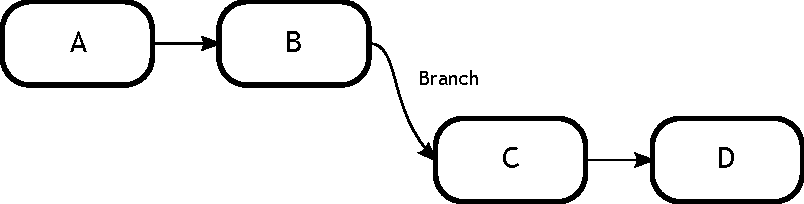
\includegraphics[width=9cm]{images/f-w7-d2.pdf}
\caption{Standard commit tree example}
\end{figure}

Now what will inevitably happen is that some more development will continue in the source project, which is represented in the Figure below by commits \textbf{E} and \textbf{F}.
This is shown below in Figure 3.
In our use case, we actually want these new changes to be present during our development.
Let us see how we can handle this.

\begin{figure}[hbt]
\centering
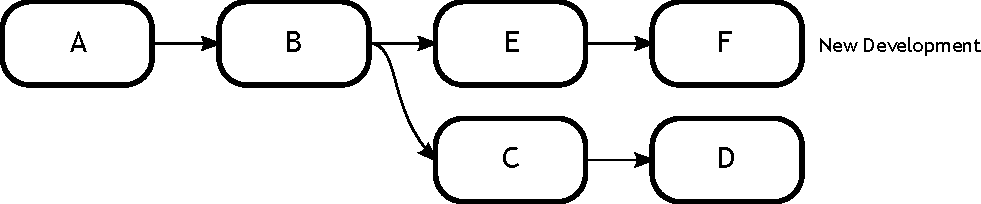
\includegraphics[width=9cm]{images/f-w7-d3.pdf}
\caption{Continued development}
\end{figure}

We could quite happily merge the \textbf{master} branch into our own, but that would result in a merge commit being added, plus the fact that as we go further down the line, our development work would be interlaced with various updates from the \textbf{master}.
A better way to handle this sometimes, is by using the rebase tool which will achieve the results displayed below in Figure 4.

\begin{figure}[hbt]
\centering
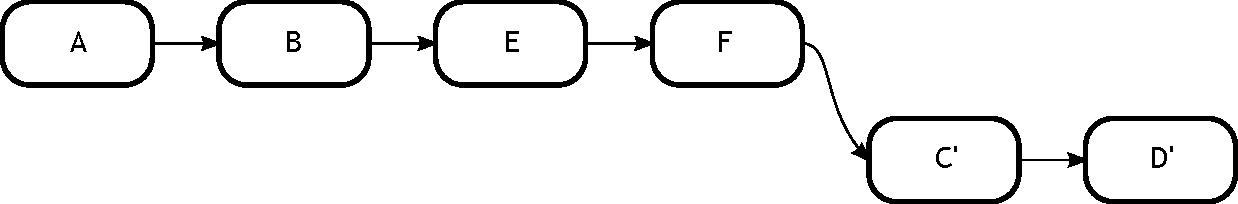
\includegraphics[width=9cm]{images/f-w7-d4.pdf}
\caption{A rebase in action}
\end{figure}

As you can see we have a slight alteration to the diagram.
Commits \textbf{C} and \textbf{D} have little ticks next to them.
This is to indicate that they are actually not the same commits as before.
You may be wondering why? Think about it for a few minutes.
In Git, every commits SHA-1 hash is based not only on the contents of that commit, but also on the parent.
In this way, if we move these commits, then their SHA-1 hashes are going to change.
Our notation is simply stating that although the contents of these commits is the same, they are the \textbf{C} and \textbf{D} that we remember, their identifier will change.

Remember our discussion about changing the past? This is very relevant here.
Rebasing is the ultimate way to change the past.
Over the next few days, we are going to demonstrate a number of ways that rebase can aid you in your development and produce a clean and structured commit history.
However, care must be taken not to rebase something which others have already pulled.
Remember, with great power, comes great responsibility.

Let us now turn out attention to actually looking at an example of the rebase tool.
We are going to take our example repository and create a branch.
Then we are going to do some work on the \textbf{master} branch and try rebasing our changes.

\section{Day 3 - ``Rebasing our commitments''}
\subsection{Rebase examples}

We are now going to go back to our \texttt{coderepo} folder.
This is the one we cloned from in Week 6 to create the \texttt{coderepo-cl} repository.
When we left this repository, we were at commit \textbf{1c3206a}.
If you have played with the repository at all, it would be a good opportunity for you to bring the wonderful branch to that point.
We are also going to Fast Forward the master branch to that same point to.
Before reading on, try to remember what commands we would use to do this and then check below to see if you are right.

\begin{code}
john@satsuki:~/coderepo$ git checkout wonderful
Already on 'wonderful'
john@satsuki:~/coderepo$ git reset --hard 1c3206a
HEAD is now at 1c3206a Added a new file
john@satsuki:~/coderepo$
\end{code}

So we begin by ensuring that we are on the \textbf{wonderful} branch.
Then we perform a hard reset, to ensure that the HEAD of \textbf{wonderful} points to the commit \textbf{1c3206a}.

\begin{code}
john@satsuki:~/coderepo$ git checkout master
Switched to branch 'master'
john@satsuki:~/coderepo$ git merge wonderful
Updating 37950f8..1c3206a
Fast-forward
 newfile3 |    1 +
 1 files changed, 1 insertions(+), 0 deletions(-)
 create mode 100644 newfile3
john@satsuki:~/coderepo$
\end{code}

Next we use the \texttt{git merge} command as before to bring the \textbf{master} branch in line with the \textbf{wonderful} branch.
As there have been no more commits to \textbf{master} since we worked on \textbf{wonderful}, it means that once again, the merge can be a simple Fast Forward merge, allowing us to simple change which commit HEAD points to within the \textbf{master} branch.

\begin{code}
john@satsuki:~/coderepo$ git branch -v
  master    1c3206a Added a new file
* wonderful 1c3206a Added a new file
  zaney     7cc32db Made another awesome change
john@satsuki:~/coderepo$
\end{code}

Finally, we run a \texttt{git branch} command to confirm that the branches point to the same commit.
Remember there are other ways we could have achieved this, using \texttt{git log} for example.
Now that we can see they point to the same place, we can continue with our introduction to the \indexgit{rebase} command.
We will start by making some commits to the \textbf{wonderful} branch and see how we can update our underlying master branch.

\begin{code}
john@satsuki:~/coderepo$ echo "New Changes" >> another_file
john@satsuki:~/coderepo$ git commit -a -m 'Updated another file'
[wonderful c0e2f5b] Updated another file
 1 files changed, 1 insertions(+), 0 deletions(-)
john@satsuki:~/coderepo$ echo "More New Changes" >> another_file
john@satsuki:~/coderepo$ git commit -a -m 'Updated another file'
[wonderful 8c6a66b] Updated another file
 1 files changed, 1 insertions(+), 0 deletions(-)
john@satsuki:~/coderepo$ echo "More Super New Changes" >> another_file
john@satsuki:~/coderepo$ git commit -a -m 'Updated another file again'
[wonderful b91ec84] Updated another file again
 1 files changed, 1 insertions(+), 0 deletions(-)
john@satsuki:~/coderepo$ gitk --all
john@satsuki:~/coderepo$
\end{code}

Before we continue, there is a problem in the trenches.

\begin{trenches}
``Ahh dang it'' shouted Simon.
``That's really not very helpful to anyone.''

``What's up?'' said Martha over the cubicle wall.
She stood up, knocking a pile of papers over that were hanging precariously on the edge of the desk.
They scattered across the floor creating a white dividing line down the middle of the office.
She mutter something under her breath.
John and Simon began to help tidy the papers up whilst Simon started stating his problem.

``Well, I commit two commits that used the same commit message, I really wasn't thinking. Plus the fact that they should really have been one commit.''

``Just reset back and do the work again,'' shouted an eavesdropping Klaud unhelpfully.
A round of raised eyebrows circled the paper-stackers.

``You could use rebase.'' Martha was standing next to the desk now and was arranging the stack in a more suitable position on the desk.

``How so?'' John looked at Martha inquisitively.

Martha giggled.
``Rebase can do a lot more than just replaying commits you know. Some of the more simpler tasks are \ldots well \ldots let me show you.''
\end{trenches}

\index{rebasing!interactive}Looking at our example commits, it would appear that we have made the same mistake as Simon.
Our commits, \textbf{c0e2f5b} and textbf{8c6a66b} have got the same commit message.
Not very helpful at all.
Let us see how \texttt{git rebase} can help us out here.

\begin{code}
john@satsuki:~/coderepo$ git rebase -i HEAD~3
\end{code}

We have told Git to run the \texttt{rebase} command using the \texttt{-i} parameter.
This will put Git into \emph{interactive} mode.
We have also asked Git to rebase the last three commits.
The \texttt{HEAD~3} is used like before to tell us to go back three commits from the HEAD references.
When we run this command, we are presented with a text file in our default text editor.

\begin{code}
pick c0e2f5b Updated another file
pick 8c6a66b Updated another file
pick b91ec84 Updated another file again

# Rebase 1c3206a..b91ec84 onto 1c3206a
#
# Commands:
#  p, pick = use commit
#  r, reword = use commit, but edit the commit message
#  e, edit = use commit, but stop for amending
#  s, squash = use commit, but meld into previous commit
#  f, fixup = like "squash", but discard this commit's log message
#  x, exec = run command (the rest of the line) using shell
#
# If you remove a line here THAT COMMIT WILL BE LOST.
# However, if you remove everything, the rebase will be aborted.
#
\end{code}

At the top of the file, you can see the last three commits, along with their commit message, prefixed by the word pick.
We will get to what this really means in a few minutes, but as you can see there are a large number of options within the rebase interactive system.
If we closed the file and left it unchanged, the rebase would end without altering anything.
The options are fairly self explanitory but they allow us to change many elements of a commit or a series of commits.

In our case, we can use this to reword the second commit, \textbf{8c6a66b}.
We are going to modify the lines above to look like the ones below.

\begin{code}
pick c0e2f5b Updated another file
r 8c6a66b Updated another file
pick b91ec84 Updated another file again
\end{code}

\index{rebasing!editing messages}Notice that we replaced the beginning of the second line, original starting with \texttt{pick}, with the letter \texttt{r}.
Using the list of available functions above, we can easily see that the \texttt{r} corresponds to the \emph{reword} function, which will allow us to change the wording that we have used for that particular commit.
On saving this and closing this file, Git quickly presents us with another editor window.
This time the window contains a more familiar commit message setup.
We will modify it to show the same as below, and then close the editor.

\begin{code}
Updated another file 2nd time

# Please enter the commit message for your changes. Lines starting
# with '#' will be ignored, and an empty message aborts the commit.
# Not currently on any branch.
# Changes to be committed:
#   (use "git reset HEAD^1 <file>..." to unstage)
#
#       modified:   another_file
#
# Untracked files:
#   (use "git add <file>..." to include in what will be committed)
#
#       temp_file
\end{code}

After Git completes working on the rebase, we are presented with the result of our operation.

\begin{code}
john@satsuki:~/coderepo$ git rebase -i HEAD~3
[detached HEAD 7c35dde] Updated another file 2nd time
 1 files changed, 1 insertions(+), 0 deletions(-)
Successfully rebased and updated refs/heads/wonderful.
john@satsuki:~/coderepo$
\end{code}

So Git has completed the operation, and by running an abbreviated \texttt{git log} command, we can see that the fruits of our labour have resulted in the second commit having its working changed.

\begin{code}
john@satsuki:~/coderepo$ git log --graph --pretty=oneline --all --abbrev-commit --decorate -n 4
* aeb5679 (HEAD, wonderful) Updated another file again
* 7c35dde Updated another file 2nd time
* c0e2f5b Updated another file
* 1c3206a (master) Added a new file
john@satsuki:~/coderepo$
\end{code}

\begin{callout}{Note}{Rebasing and the hashes}
If you have been paying attention to the SHA-1 hashes as we have been moving through this last piece on rebasing, you may have noticed something interesting.
Though there are commits that we have not altered at all, the commit IDs have indeed changed.
If we take the example where we re-worded the second commit, it is clear to see that subsequent commits have their IDs changed.
In the example, we modified commit \textbf{8c6a66b}, but we left \textbf{b91ec84} untouched.
In the resulting tree, both have had their IDs changed.
\newline
\newline
The reason for this is simple, remember we are replaying commits.
In a sense we are re-committing the changes that were made during that commit.
As we have stated previously, Git is cryptographically secure.
By this we mean that each commit relies on the commit that preceeds it.
So, if we change the ID of a preceeding commit, all subsequent ones have to change also.
\end{callout}

Let us try this rebase again.
This time we will use the sqush option to merge the two similar commits into one.
We will run the same command as before; \texttt{git rebase -i HEAD\textasciitilde3}.
This time we will use the \texttt{s} prefix to the line to choose \emph{squashing} as our method.
We could have used the word \texttt{sqush} instead of \texttt{s}, but for the laziness in all of us, we will opt for the single letter versions for now.

\begin{code}
pick c0e2f5b Updated another file
s 7c35dde Updated another file 2nd time
pick aeb5679 Updated another file again

# Rebase 1c3206a..aeb5679 onto 1c3206a
\end{code}

\index{rebasing!squashing}Now when we save and close the file, we are presented with a slightly different screen.
As we are squashing several commits together into one, we need to choose a commit message.
The message needs to be descriptive enough that it will accturately let a developer see what has been updated in this single commit.
We will delete these lines and replace them with the comment \texttt{Updated another file with 2 edits}.

\begin{code}
# This is a combination of 2 commits.
# The first commit's message is:

Updated another file

# This is the 2nd commit message:

Updated another file 2nd time
\end{code}

After completion, Git shows us that the rebase has been successful.

\begin{code}
[detached HEAD 1ffe37f] Updated another file with 2 edits
 1 files changed, 2 insertions(+), 0 deletions(-)
Successfully rebased and updated refs/heads/wonderful.
john@satsuki:~/coderepo$
\end{code}

By using the \texttt{git log} message, we can see that the two commits have indeed been replaced by one.

\begin{code}
john@satsuki:~/coderepo$ git log --graph --pretty=oneline --all --abbrev-commit --decorate -n 4
* 4d91aab (HEAD, wonderful) Updated another file again
* 1ffe37f Updated another file with 2 edits
* 1c3206a (master) Added a new file
* 37950f8 Continued Development
john@satsuki:~/coderepo$
\end{code}

\begin{trenches}
``Actually that's pretty cool,'' commented Simon, after Martha had shown him how to use rebase to squash and reword.
She smiled, but said nothing.
Martha had an uncanny knack for knowing when there was going to be another question.
``So, just how would we use git rebase for keeping a development tree up to date?''

Martha ruffled Simon's hair.
She liked his youthful enthusiasm.
``How about we take a crack at that tomorrow eh?''
\end{trenches}

\section{Day 4 - ``Starting to get rebased''}
\subsection{Using rebase with branches}

\index{continuous integration}Up until now we have used \texttt{git rebase} to work on our current branch, modifying a few things here and there.
This is actually one of the simplest things that rebase can perform, and as hinted to in our workflow design, we can actually use \texttt{git rebase} to perform something called \emph{Continuous Integration}.

As we stated before, one of the most interesting uses of using \texttt{git rebase} is to update your branch with changes from another, whilst keeping your development intact.
The great part about it is that there is no messy merging, your commits appear at the end of the tree which makes things nice and tidy.
Let us go back to our example and add some more commits to the \textbf{master} branch.

\begin{code}
john@satsuki:~/coderepo$ git checkout master
Switched to branch 'master'
john@satsuki:~/coderepo$ touch cont_dev
john@satsuki:~/coderepo$ echo "New info" >> cont_dev
john@satsuki:~/coderepo$ git add cont_dev
john@satsuki:~/coderepo$ git commit -a -m 'Start new dev'
[master 1968324] Start new dev
 1 files changed, 1 insertions(+), 0 deletions(-)
 create mode 100644 cont_dev
john@satsuki:~/coderepo$ echo "A cool function" >> cont_dev
john@satsuki:~/coderepo$ git commit -a -m 'Finished new dev'
[master f8d5100] Finished new dev
 1 files changed, 1 insertions(+), 0 deletions(-)
john@satsuki:~/coderepo$ git logg -n5
* f8d5100 (HEAD, master) Finished new dev
* 1968324 Start new dev
| * 4d91aab (wonderful) Updated another file again
| * 1ffe37f Updated another file with 2 edits
|/
* 1c3206a Added a new file
john@satsuki:~/coderepo$
\end{code}

You may have noticed that we seem to have introduced a new command here called \texttt{git logg}.
The command seems to do exactly the same as our \texttt{git log --graph --pretty=oneline --all --abbrev-commit --decorate} command.
For more information about what we have done here, see the callout called \textbf{An alias in our midst}.

\begin{callout}{Information}{An alias in our midst}
\index{aliases}Some times, you will get tired of typing the same old long string of parameters into Git.
Though some people tend to frown upon using them, aliases can significantly increase your productivity, by allowing you to shortcut annoyingly long commands.
You may have noticed our \texttt{git log --graph --pretty=oneline --all --abbrev-commit --decorate} command from before.
It is awfully long.
Let us create an alias called \texttt{git logg}.

There are multiple ways to do this, but we are going to get a little down and dirty and edit the \texttt{.git/config} file in our repository.
You will find a few \emph{stanzas} which start like this \texttt{[core]}, followed by a number of lines.
If you don't already have one, use the editor to add \texttt{[alias]} at the end of the file, so that your file has a section looking like the following.

\begin{code}
[alias]
        logg = log --graph --pretty=oneline --all --abbrev-commit --decorate
\end{code}

Once saved, we can use \texttt{git logg} just like any other Git command.
As you can see from the example in the text, we can even append more parameters that the parent command \texttt{git log} usually accepts.
So we can do things like \texttt{git logg -n5} to get only five entries.
\end{callout}

So we have two development trees, our \textbf{master} which is what our development work is based on, and our \textbf{wonderful} branch, which is where we are performing our development work.
The task now is to update the \textbf{wonderful} branch, with all of the changes that have taken place in \textbf{master}.
To do this, we use the \texttt{git rebase} tool once more, but this time in a slightly different manner.

\begin{code}
john@satsuki:~/coderepo$ git checkout wonderful
Switched to branch 'wonderful'
john@satsuki:~/coderepo$ git rebase master
First, rewinding head to replay your work on top of it...
Applying: Updated another file with 2 edits
Applying: Updated another file again
john@satsuki:~/coderepo$ git logg -n5
* 5167cce (HEAD, wonderful) Updated another file again
* 551086e Updated another file with 2 edits
* f8d5100 (master) Finished new dev
* 1968324 Start new dev
* 1c3206a Added a new file
john@satsuki:~/coderepo$
\end{code}

We started by checking out the \textbf{wonderful}.
With the \texttt{git rebase master} command, we told Git to take all of the changes in our topic branch called \textbf{wonderful}, and replay them on top of the new \textbf{master}.
We could have also used the command \texttt{git rebase master topic} which would actually have done the original \texttt{git checkout} for us.

\index{rebasing!continuing}\index{rebasing!aborting}Notice again, that our commit IDs have changed.
The contents, in this case, remain identical, as we have not hit upon any conflicts during out rebase.
If we had, we would have to have resolved that, and then run the \texttt{git rebase --continue}, or \texttt{git rebase --abort} to abort the rebase completely.

So, our wonderful branch is now sat on top of the new development changes and instead of having two diverging branch heads, we now have a single branch which \textbf{wonderful} extends from.

\begin{trenches}
``Martha!'' Simon shouted across the office at the seemingly new Git expert.
``HELP!!''

Martha got up from her seat.
It hadn't been fifteen minutes since she had shown Simon how to rebase branches and now he was calling her again.
At first she had tried to ignore it, but the waves of SOS had plunged through the headphones and reverberated round her head one too many times.
She placed the music on hold and put the headphones on the desk.

``What's up Simon?'' she asked, smiling at John who was chuckling to himself at his desk.

``Well, I kinda rebased, but I wish I hadn't now, cos it all went wrong. How can I go back?''
\end{trenches}

\index{rebasing!undoing}It's an interesting question.
How would we move back again? We have rewritten history, how could we possibly hope to go back again? We have discussed before how most things in Git are never really immediately gone, even if we delete them.
Does this apply here too? Of course it does.
Remember that a branch is really just defined by which commit the HEAD points to.
Let us draw a few diagrams to show how the tree of commits looks before and after our rebase.

\begin{figure}[hbt]
\centering
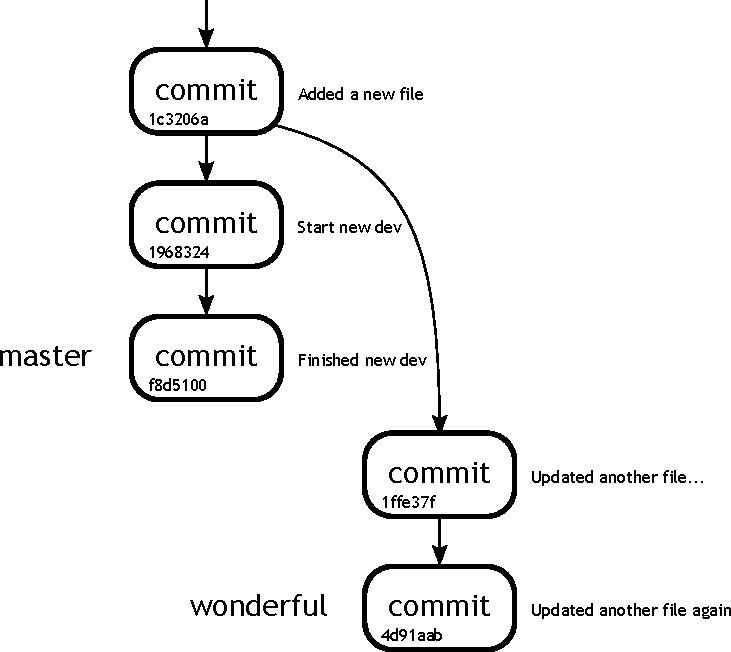
\includegraphics[width=9cm]{images/f-w7-d5.pdf}
\caption{Our repository before the rebase}
\end{figure}

Figure 5 shows our repository before we perform the rebase.
We can quite clearly see that there are two branches, diverging from the common ancestor, \textbf{1c3206a}.
In Figure 6, we see the repository after the rebase has taken place.
Notice that the two commits that \emph{were} forming the \textbf{wonderful} branch are now coloured in grey.

\begin{figure}[hbt]
\centering
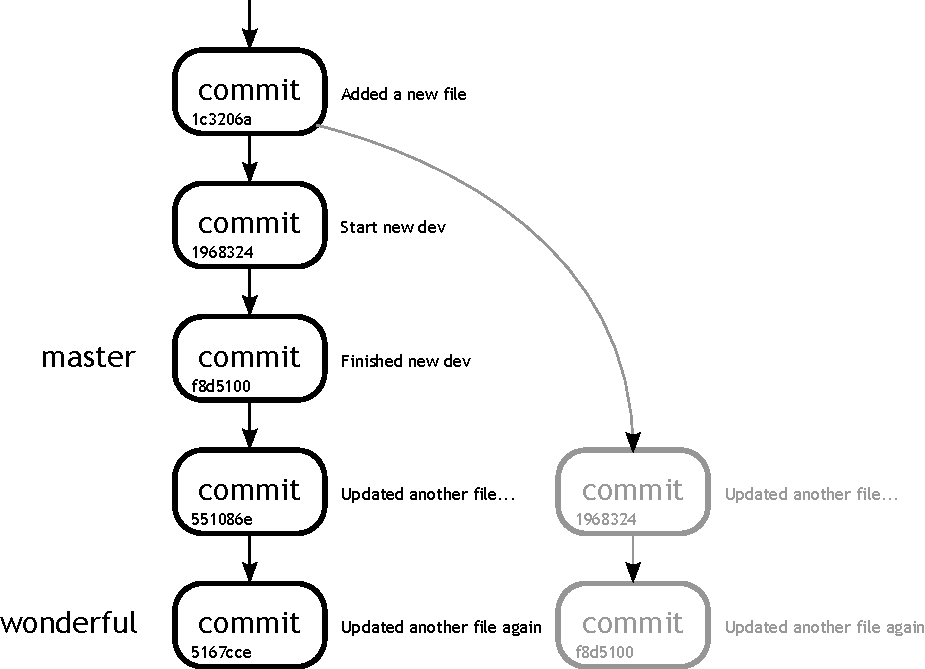
\includegraphics[width=9cm]{images/f-w7-d6.pdf}
\caption{Our repository after the rebase}
\end{figure}

\index{dangling}The grey commits are no longer referenced.
No branche HEADs point to them, and no other commits rely upon them.
In short they have been orphaned, or are left \index{dangling}\emph{dangling}.
A dangling commit has no references left pointing to it.
Remember each commit relies on its parent.
Therefore because the HEAD of \textbf{wonderful} now points to \textbf{5167cce}, and that in turn points to \textbf{551086e}.
The original commit line is unchanged.

Thinking back to previous weeks, we have had a similar situation before.
If we know the commit ID that we wish to return to, there really is nothing more complicated than issuing a \texttt{git reset}.
The only tricky part is knowing the commit you wish to return to.

\index{reflog}We do however have a weapon at our disposal.
The \texttt{git log} tool can be used with the \texttt{-g}.
This parameter forces the Git to refer to the \emph{reflog} for entries, instead of traversing the usualy tree.
If you remember, the reflog is our key to seeing what happened in the past.
It holds a list of all the previous HEADs of each branch.
By supplying the branch name, we can see everything that happened to the \textbf{wonderful} branch.

\begin{code}
john@satsuki:~/coderepo$ git log -g wonderful -n2
commit 5167cce7864ca71420ce5dc37ec9b3f931727db3
Reflog: wonderful@{0} (John Haskins <john.haskins@tamagoyakiinc.koala>)
Reflog message: rebase finished: refs/heads/wonderful onto f8d5100142b43ffaba9bb
Author: John Haskins <john.haskins@tamagoyakiinc.koala>
Date:   Wed Jul 6 09:30:40 2011 +0100

    Updated another file again

commit 4d91aab57aaad020e62486805e25d0d6f06fdc3e
Reflog: wonderful@{1} (John Haskins <john.haskins@tamagoyakiinc.koala>)
Reflog message: rebase -i (finish): refs/heads/wonderful onto 1c3206a
Author: John Haskins <john.haskins@tamagoyakiinc.koala>
Date:   Wed Jul 6 09:30:40 2011 +0100

    Updated another file again
john@satsuki:~/coderepo$
\end{code}

As you can see, the log shows that we recently completed two rebases.
The first resulted in an ID of \textbf{4d91aab} and the second resulted in \textbf{5167cce}.
As it happens, we are trying to get back to the end of that first rebase, before we ran the second.
So if we run the reset against that ID, we should return to our pre-rebased state.

\begin{code}
john@satsuki:~/coderepo$ git reset --hard 4d91aab
HEAD is now at 4d91aab Updated another file again
john@satsuki:~/coderepo$ git logg -n5
* f8d5100 (master) Finished new dev
* 1968324 Start new dev
| * 4d91aab (HEAD, wonderful) Updated another file again
| * 1ffe37f Updated another file with 2 edits
|/
* 1c3206a Added a new file
john@satsuki:~/coderepo$
\end{code}

As you can see, even though the commit messages are identical, the history of them differs.
Obviously now, it is our rebased version which is left dangling and if it continues to go unused, it will eventually be deleted.
Of course it is also possible to create a branch to point to the dangling commit.
In this way it would never get deleted.
Let us just see how we could achieve this.

Armed with the knowledge that the commit we are looking for is \textbf{5167cce}, we can run the \texttt{git branch} command and specify a starting point.

\begin{code}
john@satsuki:~/coderepo$ git branch keeprebase 5167cce
john@satsuki:~/coderepo$ git branch -v
  keeprebase 5167cce Updated another file again
  master     f8d5100 Finished new dev
* wonderful  4d91aab Updated another file again
  zaney      7cc32db Made another awesome change
john@satsuki:~/coderepo$ git logg -n7
* 5167cce (keeprebase) Updated another file again
* 551086e Updated another file with 2 edits
* f8d5100 (master) Finished new dev
* 1968324 Start new dev
| * 4d91aab (HEAD, wonderful) Updated another file again
| * 1ffe37f Updated another file with 2 edits
|/
* 1c3206a Added a new file
john@satsuki:~/coderepo$
\end{code}

\begin{figure}[hbt]
\centering
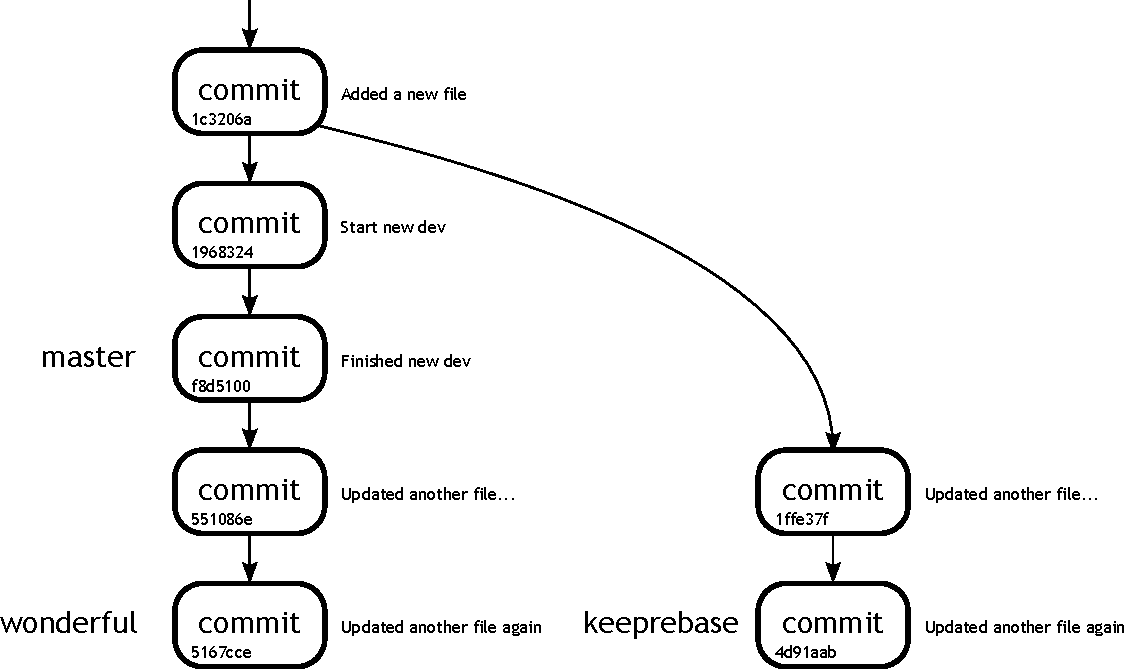
\includegraphics[width=9cm]{images/f-w7-d7.pdf}
\caption{Our repository after the recovery}
\end{figure}

Notice our branch is now created and looking at the log, it contains the same two commits and the tree looks as we would expect.
We have our \texttt{another\_file} updates in both branches.

\section{Day 5 - ``I could rebase the world''}
\subsection{Migrating commits}

We are almost at the end our our journey with the rebase tool and have one more stop before we start looking at other features of Git.

\begin{trenches}
Rob was sitting with his head on the table.
Every few seconds he would lift it up before thumping it down again.
It was obvious to everyone in the office that Rob had done something wrong.
In the end it was John who broke the rhythmic bass drum.
He pulled up a chair next to the desk.

``Come on Rob,'' started John, ``What's eating you?''

``Well, I have been working away, committing to a branch, but it wasn't the right one.''
He looked like he was almost in tears.

John frowned, ``Can't you just move a new branch forward and then rewind the other one?''

``No.'' His voice was tired and weary.
``The ancestor of the branch isn't right. I thought I had branched from master, but I'd actually branched from a dev branch. Now I can't find a way to bring my commits back. Short of cherry picking each one, but I have over fifty of them. Guess it's time to start scripting.''

John smiled and shook his head, ``Don't worry Rob, I have a better plan''
\end{trenches}

\index{cherry picking}Cherry picking is a method of copying the contents of one commit into another and is something that we will pick up on later, but we will first look at our final use of rebase.
Imagine the scenario painted above.
You made a branch, have been merrily committing for hours, before realising that actually you branched from the wrong place.

In Git, this isn't a problem.
Things get complicated if you've been doing more advanced operations during this period, but if you have been simply adding commits, we can use rebase to migrate that tree of commits to a different ancestor.

Take the example we have been working on, currently we have a \textbf{master} branch and a \textbf{wonderful} branch, and these differ.
Let us say we are currently sitting on the \textbf{wonderful} branch, but we thought we were on the \textbf{branch} and we created a new branch called develop.

\begin{code}
john@satsuki:~/coderepo$ git checkout -b develop
Switched to a new branch 'develop'
john@satsuki:~/coderepo$
\end{code}

Now let us commit a few files and see what we can do about fixing our problem.

\begin{code}
john@satsuki:~/coderepo$ echo "new dev work" >> newfile3
john@satsuki:~/coderepo$ git commit -a
[develop eb7f633] Some new dev work
 1 files changed, 1 insertions(+), 0 deletions(-)
john@satsuki:~/coderepo$ echo "newer dev work" >> newfile2
john@satsuki:~/coderepo$ git commit -a
[develop 5e0964b] More new deving
 1 files changed, 1 insertions(+), 0 deletions(-)
john@satsuki:~/coderepo$
\end{code}

Let us use our little log alias and see the work we just did on our \textbf{"master"} branch.

\begin{code}
john@satsuki:~/coderepo$ git logg -n8
* 5e0964b (HEAD, develop) More new deving
* eb7f633 Some new dev work
* 4d91aab (wonderful) Updated another file again
* 1ffe37f Updated another file with 2 edits
| * 5167cce (keeprebase) Updated another file again
| * 551086e Updated another file with 2 edits
| * f8d5100 (master) Finished new dev
| * 1968324 Start new dev
|/
john@satsuki:~/coderepo$
\end{code}

Whoops! The commits were supposed to be on a branch that stemmed from \textbf{master}, not one that stems from \textbf{wonderful}.
This is where \texttt{git rebase} comes to our assistance once more.
With one command, we can move those commits to a branch that stems from \textbf{master}.

\begin{code}
john@satsuki:~/coderepo$ git rebase --onto master wonderful develop
First, rewinding head to replay your work on top of it...
Applying: Some new dev work
Applying: More new deving
john@satsuki:~/coderepo$ git logg -n8
* aed985c (HEAD, develop) More new deving
* af3c6d7 Some new dev work
| * 5167cce (keeprebase) Updated another file again
| * 551086e Updated another file with 2 edits
|/
* f8d5100 (master) Finished new dev
* 1968324 Start new dev
| * 4d91aab (wonderful) Updated another file again
| * 1ffe37f Updated another file with 2 edits
|/
john@satsuki:~/coderepo$
\end{code}

Notice in the output above that we have used our \texttt{git rebase} tool with a new \texttt{--onto master} parameter.
Basically the syntax is stating that we would like to take the commits between \textbf{wonderful} and \textbf{develop} and place them onto \textbf{master} instead.

To clean up our repository, we are going to delete our \textbf{keeprebase} branch.

\begin{code}
john@satsuki:~/coderepo$ git branch -D keeprebase
Deleted branch keeprebase (was 5167cce).
john@satsuki:~/coderepo$
\end{code}

We have reached the end of our tour with the rebase tool.
It is exceedingly powerful and is definitely one of the tools that you should understand before using.
As stated before, do not forget the fact that rebasing changes history.
In all cases that we have used rebase, commit IDs have been changed and therefore you must be very careful when using it.

\clearpage

\section{Summary - John's Notes}
\subsection{Commands}
\begin{itemize}

\item\texttt{git rebase -i HEAD~3} - Runs the rebase tool interactively for the last three commits

\item\texttt{git rebase <branchA> <branchB>} - Lift all commits between the common ancestor of branchA and branchB and replay them on top of branchB

\item\texttt{git branch <branch\_name> <startpoint>} - Create a new branch starting from a definte start point

\item\texttt{git rebase --onto master <branchC> \newline <branchA> <branchB>} - Lift all commits between the common ancestor of branchA and branchB and replay them on top of branchC
\end{itemize}

\subsection{Terminology}
\begin{itemize}
\index{Terminology!SSH}\item\textbf{SSH} - A type of secure network protocol
\index{Terminology!HTTP}\item\textbf{HTTP} - The protocol that is used to serve internet pages
\index{Terminology!Rebase}\item\textbf{Rebase} - Used primarily for lifting commits and reapplying them to another base branch
\end{itemize}
